\chapter{Proposed Methodology}
In this chapter we will discuss about our proposed methodology and learn about every module of our system. We will find short mathematical insight of each learning algorithm used in our system. Finally overall system is summarized with an example.

\section{Proposed Text Classification System}
The key objective of our project is to design a system that can classify suspicious and non-suspicious text. \textbf{Fig} \ref{fig:proposed_model} shows an abstract view of our system.
\vspace{0.5cm}
\begin{figure}[h!]
\centering
  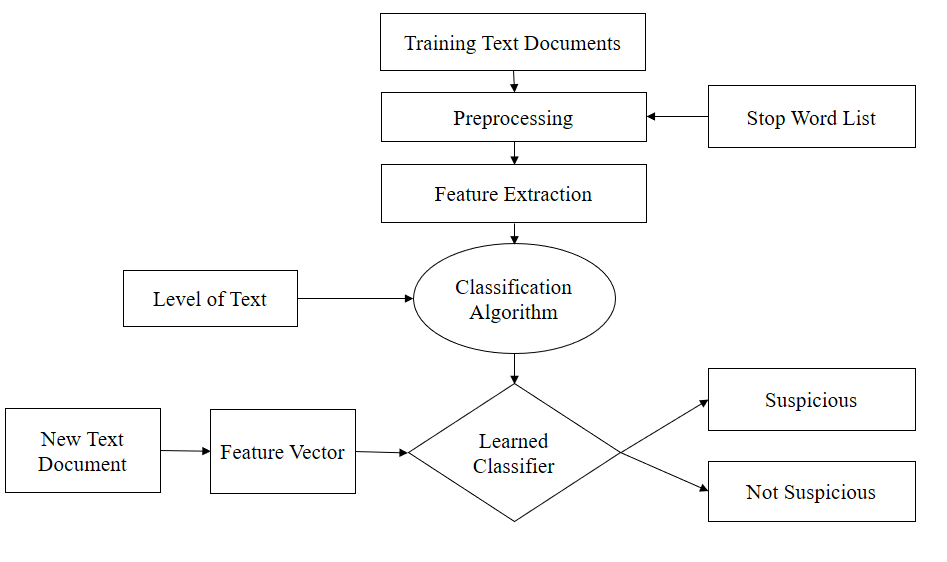
\includegraphics[scale=0.6]{Figures/proposed_model.PNG}
  \caption{Proposed Model of Suspicious Text Detection}
  \label{fig:proposed_model}
\end{figure}
 
 \section{Training Text Corpus}
 Supervised learning involves using a set of training examples that make up the training data. In linguistics, a corpus or text corpus is a large and structured set of texts nowadays usually electronically stored and processed. For a machine learning algorithm a well corpus is essential to perform according to expectation. In the corpus each training example consists of an input text and desired output value. An algorithm is then applied to the data to produce a classifier which will determine the correct output for any further valid input values. In Bengali language processing there is no corpus available which contains suspicious text. But as ours is a supervised classification system, our suspicious text detector needs a training corpus which consist of text and labels indicating whether a text is suspicious or non-suspicious. To implement this system we collect a large amount of Bangla  suspicious text. This texts are collected from online blogs, newspaper, Facebook post and other type of electronic source. Training corpus is divided into positive set (Suspicious text) and negative set (non-suspicious text). The accuracy of the learning algorithms depend on uniqueness of training examples.
 
 \section{Preprocessing}
 In natural language processing, data preprocessing is an essential step. Data preprocessing is a data mining technique that involves transforming raw data into an understandable format. Real world data is often incomplete, inconsistent, and/or lacking in certain behaviors or trends, and is likely to contain many errors. Data preprocessing is a proven method of resolving such issues. Data preprocessing is required to fill in missing values, smooth noisy data, identify or remove the outliers, and resolve inconsistencies.
 Words with no significance must be removed from the text. In our system all texts are preprocessed by the preprocessor. We use main bodies of the text to train suspicious text detector. We are going to represent our text document by list of words and their frequencies. We have a stop word list which consist of words that make no contribution to classify text. In our preprocessing section, such word will be removed by matching with stop word list. It will be very helpful to increase efficiency of the system because redundant will slow our system and increase computational complexity of the system.
 
\section{Feature Extraction}
Word frequencies will be used as feature in our proposed system. Word frequencies are used as features quite often, and although they are usually considered a basic feature, they can prove to be effective.
Terms associated with feature extraction of our system are described shortly.
\subsection{CountVectorizer}

CountVectorizers used to learn the vocabulary of a set of texts and then transform them into a data-frame that can be used for building models. CountVectorizer takes few parameter that is important for extracting feature accurately.

\subparagraph{Stop Words :}
CountVectorizer just counts the occurrences of each word in its vocabulary, extremely common words stop words will become very important features while they add little meaning to the text. In our system we do not take those words into account which improves system accuracy.
\subparagraph{Min-DF, Max-DF :}
These parameters are the minimum and maximum document frequencies words/n-grams must have to be used as features. If either of these parameters are set to integers, they will be used as bounds on the number of documents each feature must be in to be considered as a feature. If either is set to a float, that number will be interpreted as a frequency rather than a numerical limit.
\subparagraph{Max-Features :}
\texttt{max\_features} parameter is used to limit maximum number of feature used by the model. In our system we take most frequent 1000 words by using this parameter to reduce time and storage complexity.

\subsection{Word2vec}
Word2vec is used to train different learning model. Word2vec takes as its input a large corpus of text and produces a vector space, typically of several hundred dimensions, with each unique word in the corpus being assigned a corresponding vector in the space. Word vectors are positioned in the vector space such that words that share common contexts in the corpus are located in close proximity to one another in the space. Accuracy increases overall as the number of words used increases, and as the number of dimensions increases. But we should be careful about associated complexities. 

\subsection{TF-IDF}
The tf–idf is the product of two statistics, term frequency and inverse document frequency. There are various ways for determining the exact values of both statistics.

\subparagraph{Term Frequency}$tf(t,d)$, the simplest choice is to use the raw count of a term in a document, i.e., the number of times that term $t$ and occurs in document $d$.If we denote the raw count by $f_{t,d}$, then the simplest $tf$ scheme is $tf(t,d) = f_{t,d}$. Term frequencies can be calculated in  different ways,
\begin{enumerate}
    \item Term Frequency : 
    \begin{equation}
        \dfrac{f_{t,d}}{\sum_{t'\epsilon d}^{}f_{t',d}}
    \end{equation}
    \item Logarithmically scaled frequency :
    \begin{equation}
         tf(t,d)=\log(1+f_{t,d})
    \end{equation}
   
    \item To prevent bias for longer documents following equation is used:
    \begin{equation}
        tf(t,d) = 0.5 + 0.5 * \frac{f_{t,d}}{\max{(f_{t',d}\colon t'\epsilon d)}}
    \end{equation}
\end{enumerate}

\subparagraph{Inverse Document Frequency}
is a measure whether a term is common or rare across all document. IDF can be calculated by following equation,
\begin{equation}
    idf(t,d) = \log \frac{N}{\abs{1+(d\epsilon D\colon t\epsilon d)}}
\end{equation}
\noindent
%\vspace{0.5cm}
$N$ : Total number of documents in the corpus $N = \abs{D}$\newline
$(d \epsilon D\colon t\epsilon d)$ : \textrm{Number of document where term $t$ appears.}\newline
\vspace{0.5cm}
Now $tf-idf$ is calculated as,
\begin{equation}
    tfidf(t, d, D) = tf(t, d)*idf(t, D)
\end{equation}
So, Final weighting scheme of $tf-idf$ is,
\begin{equation}
        tfidf(t, d, D)=(0.5 + 0.5 * \frac{f_{t,d}}{\max{(f_{t',d}\colon t'\epsilon d)}})*\log \frac{N}{n_t}
\end{equation}
\clearpage

\section{Classification Algorithm}
After extracting feature from the text, now these features are used to train our machine learning model. Different classification algorithms have been used for training purpose.

\subsection{Naive Bayes Classifier}
Naive Bayes is a simple technique for constructing classifiers using feature values. All naive Bayes classifiers assume that the value of a particular feature is independent of the value of any other feature, given the class variable. \textbf{Fig} \ref{fig:NBC} shows decision boundary for Naive Bayes classifier.

\begin{figure}[h!]
    \centering
    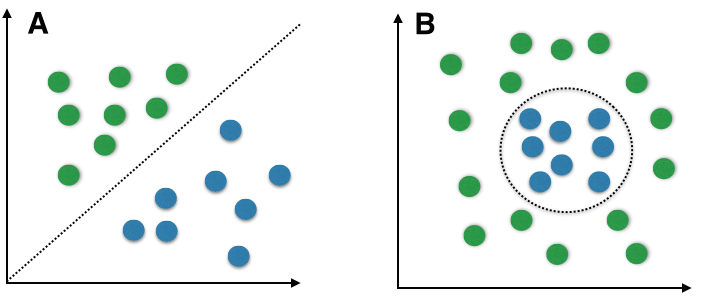
\includegraphics[scale=0.4]{Figures/naive_bayes.png}
    \caption{Naive Bayes Classifier}
    \label{fig:NBC}
\end{figure}

%%% Citation ache %%%%%%
As a popular classification algorithm, Naive Bayes algorithm [4] will be used in our system. It can be defined as Bayes theorem with a conditional independency assumption that all variables $A_{1},A_{2},...,A_{n}$ in a given category $C$ are conditionally independent with each other given $C$. 
According to Bayes rule for a text document $(T)$ and class $(C)$ we can write,$$ P(C|T) = \frac{P(T|C)P(C)}{P(T)}$$
The class we are looking for to assign this document is out of all classes the one that maximizes the probability of that class given the document.
\begin{equation}\label{eq:11}
 \begin{aligned}
     C_{MAP} & = argmax P(C|T) \\     & = argmax \frac{P(T|C)P(C)}{P(T)}\\
    & = argmax {P(T|C)P(C)}
\end{aligned}
\end{equation}
So final equation for Naive Bayes Classifier is,
\begin{equation}
     C_{MAP} = argmax P(X_{1},X_{2},...,X_{n}|C)P(C)
\end{equation}
